\documentclass[titlepage,landscape]{seminar}
\usepackage{url}
\usepackage{graphicx}
\usepackage{hyperref}
\usepackage{epstopdf}
\usepackage{slides}

\newcommand{\frack}{\frac{1}{k}}

\begin{document}

\myslide{
\heading{Mating table with complete self-fertilization}
\begin{center}
\begin{tabular}{ccccc}
\hline\hline
&&\multicolumn{3}{c}{Offsrping genotype} \\
Mating & frequency & $A_1A_1$ & $A_1A_2$ & $A_2A_2$ \\
\hline
$A_1A_1 \times A_1A_1$ & $x_{11}$ & 1 & 0 & 0 \\
$A_1A_2 \times A_1A_2$ & $x_{12}$ & $\fourth$ & $\half$ & $\fourth$ \\
$A_2A_2 \times A_2A_2$ & $x_{22}$ & 0 & 0 & 1 \\
\hline
\end{tabular}
\end{center}
\begin{eqnarray*}
x_{11}' &=& x_{11} + x_{12}/4 \\
x_{12}' &=& x_{12}/2 \\
x_{22}' &=& x_{22} + x_{12}/4 \\
\end{eqnarray*}
}

\myslide{
\heading{Offspring genotype and allele frequencies}
\begin{eqnarray*}
x_{11}' &=& x_{11} + x_{12}/4 \\
x_{12}' &=& x_{12}/2 \\
x_{22}' &=& x_{22} + x_{12}/4 \\
\end{eqnarray*}
\vfil
\begin{eqnarray*}
p' &=& x_{11}' + x_{12}'/2 \\
   &=& x_{11} + x_{12}/4 + x_{12} /4 \\
   &=& x_{11} + x_{12}/2 \\
   &=& p
\end{eqnarray*}
}

\myslide{
\heading{Partial self-fertilization}
\begin{eqnarray*}
x_{11}' &=& p^2(1-\sigma) + (x_{11} + x_{12}/4)\sigma \\
x_{12}' &=& 2pq(1-\sigma) + (x_{12}/2)\sigma  \label{eq:het} \\
x_{22}' &=& q^2(1-\sigma) + (x_{22} + x_{12}/4)\sigma
\end{eqnarray*}
\begin{eqnarray*}
\hat x_{12} &=& 2pq(1-\sigma) + (\hat x_{12}/2)\sigma \\
\hat x_{12}(1 - \sigma/2) &=& 2pq(1-\sigma) \\
\hat x_{12} &=& \frac{2pq(1-\sigma)}{(1-\sigma/2)}
\end{eqnarray*}
\begin{eqnarray*}
\hat x_{11} &=& p^2 + fpq \\
\hat x_{12} &=& 2pq(1-f) \\
\hat x_{22} &=& q^2 + fpq
\end{eqnarray*}
}

\myslide{
\heading{Identity by descent}
\begin{center}
\begin{tabular}{rcccc}
      &            & $A_1$ & $\rightarrow$ & $A_1$ \\
      & $\nearrow$ &       &               & \\
$A_1$ &            &       &               & \\
      & $\searrow$ &       &               & \\
      &            & $A_1$ & $\rightarrow$ & $A_1$
\end{tabular}
\end{center}
}

\myslide{
\heading{Identity by type}
\begin{center}
\begin{tabular}{rcccc}
      &            & $A_1$ & $\rightarrow$ & $A_1$ \\
      & $\nearrow$ &       &               & \\
$A_1$ &            &       &               & \\
      & $\searrow$ &       &               & \\
      &            & $A_2$ & $\rightarrow$ & $A_1$ \\
      & $\uparrow$ &       & $\uparrow$    & \\
      & mutation   &       & mutation      &
\end{tabular}
\end{center}
}

\myslide{
\heading{Genotype frequencies with inbreeding}
\begin{eqnarray*}
x_{11} &=& p^2(1-f) + fp \\
x_{12} &=& 2pq(1-f) \\
x_{22} &=& q^2(1-f) + fq
\end{eqnarray*}
\begin{eqnarray*}
x_{11} &=& p^2 + fpq \\
x_{12} &=& 2pq(1-f) \\
x_{22} &=& q^2 + fpq
\end{eqnarray*}
}

\myslide{
\heading{Population structure}
\begin{center}
\begin{tabular}{l|rrr}
\hline\hline
       & $A_1A_1$ & $A_1A_2$ & $A_2A_2$ \\
\hline
From forest & 16  & 48       & 36 \\
From meadow & 49  & 42       & 9 \\
\hline
Total       & 65  & 90       & 45 \\
\hline
\end{tabular}
\end{center}
}

\myslide{
\heading{Population structure}
\begin{center}
\begin{tabular}{l|rrr}
\hline\hline
       & $A_1A_1$ & $A_1A_2$ & $A_2A_2$ \\
\hline
From forest & 16  & 48       & 36 \\
From meadow & 49  & 42       & 9 \\
\hline
Total       & 65  & 90       & 45 \\
\hline
\end{tabular}
\end{center}


\begin{center}
\begin{tabular}{l|rrr}
\hline\hline
                            & $A_1A_1$ & $A_1A_2$ & $A_2A_2$ \\
\hline
Expected (from $p=0.55$)    & (0.3025)200 & (0.4950)200 & (0.2025)200 \\
                            & 60.5     & 99.0     & 40.5 \\
Observed (from table above) & 65       & 90       & 45 \\
\hline
\end{tabular}
\end{center}
}

\myslide{
\heading{Population structure: calculations}
\begin{center}
\begin{tabular}{l|rrr}
\hline\hline
         & $A_1A_1$       & $A_1A_2$         & $A_2A_2$ \\
\hline
Expected & $\bar p^2$     & $2\bar p\bar q$  & $\bar q^2$ \\
Observed & $\frack\sum p_i^2$ & $\frack\sum 2p_iq_i$ & $\frack\sum q_i^2$ \\
\hline
\end{tabular}
\end{center}
\begin{eqnarray*}
\frack\sum p_i^2 &=& \frack\sum (p_i - \bar p + \bar p)^2 \\
&=& \frack\sum \left((p_i - \bar p)^2 + 2\bar p(p_i - \bar p)
                            + \bar p^2\right) \\
             &=& \frack\sum (p_i - \bar p)^2 + \bar p^2 \\
             &=& \hbox{Var}(p) + \bar p^2 \label{eq:p2} \\
\frack\sum 2p_iq_i &=& 2\bar p\bar q - 2\hbox{Var}(p) \label{eq:2pq} \\
\frack\sum q_i^2   &=& \bar q^2 + \hbox{Var}(p) \label{eq:q2}
\end{eqnarray*}
}

\myslide{
\heading{Population structure: calculations}
\begin{eqnarray}
\hbox{Var}(p) &=& \left((0.4 - 0.55)^2 + (0.7 - 0.55)^2\right)/2 \\
              &=& 0.0225
\end{eqnarray}
\begin{center}
\begin{tabular}{l|rcrcr}
\hline\hline
         & Expected &   &           &   & Observed \\
\hline
$A_1A_1$ &   0.3025 & + &   0.0225  & = &   0.3250 \\
$A_1A_2$ &   0.4950 & - & 2(0.0225) & = &   0.4500 \\
$A_2A_2$ &   0.2025 & + &   0.0225  & = &   0.2250 \\
\hline
\end{tabular}
\end{center}
}

\myslide{
\heading{$F_{ST}$ and population structure}
\begin{eqnarray}
\frack\sum p_i^2 &=& \bar p^2 + F_{st}\bar p \bar q \label{eq:p2-f} \\
\frack\sum 2p_iq_i &=& 2\bar p\bar q(1 - F_{st}) \label{eq:2pq-f} \\
\frack\sum q_i^2   &=& \bar q^2 + F_{st}\bar p \bar q \label{eq:q2-f}
\end{eqnarray}
}

\myslide{
\heading{Wright's $F$-statistics}
\[
F_{it} = 1 - \frac{H_i}{H_t}
\]
\begin{eqnarray*}
1 - F_{it} &=& \frac{H_i}{H_t} \\
           &=& \left(\frac{H_i}{H_s}\right)\left(\frac{H_s}{H_t}\right) \\
           &=& (1 - F_{is})(1 - F_{st}) \quad ,
\end{eqnarray*}
}

\myslide{\scriptsize
\heading{Population structure: example}
\begin{center}
\begin{tabular}{c|rrr|c}
\hline\hline
           & \multicolumn{3}{c|}{Genotype} & \\
Population & $A_{1}A_{1}$ & $A_{1}A_{2}$ & $A_{2}A_{2}$ & $\hat p$ \\
\hline
Yackeyackine Soak     & 29 & 0 & 0 & 1.0000 \\
Gnarlbine Rock        & 14 & 3 & 3 & 0.7750 \\
Boorabbin             & 15 & 2 & 3 & 0.8000 \\
Bullabulling          & 9  & 0 & 0 & 1.0000 \\
Mt. Caudan            & 9  & 0 & 0 & 1.0000 \\
Victoria Rock         & 23 & 5 & 2 & 0.8500 \\
Yellowdine            & 23 & 3 & 4 & 0.8167 \\
Wargangering          & 29 & 3 & 1 & 0.9242 \\
Wagga Rock            & 5  & 0 & 0 & 1.0000 \\
``Iron Knob Major''   & 1  & 0 & 0 & 1.0000 \\
Rainy Rocks           & 0  & 1 & 0 & 0.5000 \\
``Rainy Rocks Major'' & 1  & 0 & 0 & 1.0000 \\
\hline
\end{tabular}
\end{center}
}

\myslide{\scriptsize
\heading{Population structure: calculations}
\begin{eqnarray*}
\bar p &=& 0.8888 \\
\hbox{Var}(p) &=& 0.02118 \\
F_{st} &=& 0.2143 \\
\hbox{Individual heterozygosity} &=& (0.0000 + 0.1500 + 0.1000 +
                                      0.0000 + 0.0000 + 0.1667 +
                                      0.1000 \\
                                 &&   + 0.0909 + 0.0000 +
                                      0.0000 + 1.0000 + 0.0000)/12 \\
                           &=& 0.1340 \\
\hbox{Expected heterozygosity} &=& 2(0.8888)(1 - 0.8888) \\
                           &=& 0.1976 \\
F_{it} &=& 1 - \frac{\hbox{Individual heterozygosity}}%
                    {\hbox{Expected heterozygosity}} \\
                  &=& 1 - \frac{0.1340}{0.1976} \\
                  &=& 0.3221 \\
       1 - F_{it} &=& (1 - F_{is})(1 - F_{st}) \\
           F_{is} &=& \frac{F_{it} - F_{st}}{1 - F_{st}} \\
                  &=& \frac{0.3221 - 0.2143}{1 - 0.2143} \\
                  &=& 0.1372
\end{eqnarray*}
}

\myslide{\small
\heading{Expectation and unbiased estimates}
\begin{eqnarray*}
\mbox{E}(k) &=& \sum_{k=1}^n k \mbox{P}(k) \\
     &=& n p \quad , \\
\end{eqnarray*}
\begin{eqnarray*}
\mbox{E}(\hat p) &=& \mbox{E}\left(\sum_{k=1}^n (k/n)\right) \\
          &=& \sum_{k=1}^n (k/n) P(k) \\
          &=& (1/n)\left(\sum_{k=1}^n k P(k)\right) \\
          &=& (1/n)(n p) \\
          &=& p \quad . \\
\end{eqnarray*}
}

\myslide{
\heading{Expectation and unbiased estimates}
\begin{eqnarray*}
\mbox{E}(\tilde H) &=& \mbox{E}\left(2\hat p (1 - \hat p)\right) \\
     &=& 2\left(\mbox{E}(\hat p) - \mbox{E}({\hat p}^2)\right) \\
     &=& \mbox{\color{red}\bf TAMO} \\
     &=& ((n-1)/n)2p(1-p) \quad . \\
\end{eqnarray*}
}

\myslide{
\heading{Nei's $G_{ST}$}
\begin{eqnarray*}
H_{i} &=& 1 - {1 \over N} \sum_{k=1}^{N} \sum_{i=1}^{m} {X_{kii}} \\
H_{s} &=& {\tilde n \over {\tilde n - 1}}
         \left[1 - \sum_{i=1}^{m} {\bar {\hat x_{i}^{2}}}
         - {H_{I} \over {2 \tilde n}}\right] \\
H_{t} &=& 1 - \sum_{i=1}^{m} {\bar x_{i}^{2}} + {H_{S} \over {\tilde n}}
          - {H_{I} \over {2 \tilde n N}} \\
G_{ST} &=& \frac{H_S}{H_T}
\end{eqnarray*}
}

\myslide{
\heading{Weir \& Cockerham's $\theta$}
\begin{itemize}

\item $x_{ijk} = 0,1$ - Indicator of whether allele $A_1$ is present
  in chromosome $i$ of individual $j$ in population $k$

\item Nested analysis of variance on indicator variables (chromosomes,
  within individuals, within populations)

\item Components of variance related to $F_{IS}$, $F_{ST}$, and
  $F_{IT}$

\end{itemize}
}

\myslide{
\heading{Estimates of $F_{ST}$}
\begin{center}
  \begin{tabular}{c|ccc}
\hline\hline
Method & $F_{is}$ & $F_{st}$ & $F_{it}$ \\
\hline
Direct            & 0.1372 & 0.2143 & 0.3221 \\
Nei               & 0.3092 & 0.2395 & 0.4746 \\
Weir \& Cockerham & 0.5398 & 0.0387 & 0.5577 \\
\hline
\end{tabular}
\end{center}
\vfill
\begin{center}
{\color{red}\bf Notation}
\end{center}
\begin{center}
\begin{tabular}{cc}
\hline\hline
Wright & Weir \& Cockerham \\
\hline
$F_{it}$ & $F$ \\
$F_{is}$ & $f$ \\
$F_{st}$ & $\theta$ \\
\hline
\end{tabular}
\end{center}
}

\myslide{
\heading{Statiscal vs. evolutionary sampling}

\begin{itemize}

\item {\it Statistical sampling} - Repeated samples from the same
  population differ from one another. For example, the sample
  frequency of an allele, $\hat p$, will differ from sample to sample
  even if the ``true'' population frequency, $p$, is always the same. 

\item {\it Genetic (or evolutionary) sampling} - We are rarely, if
  ever, interested only in the populations or loci we sampled. We are
  almost always interested in using them as ``representatives'' of all
  populations or loci that could have been sampled. In other words the
  populations and loci we actually studied are best regarded as a
  sample from the set of all comparable populations and loci that
  could have been studied.

\end{itemize}
}

\myslide{
\heading{Statiscal vs. evolutionary sampling}
\begin{center}
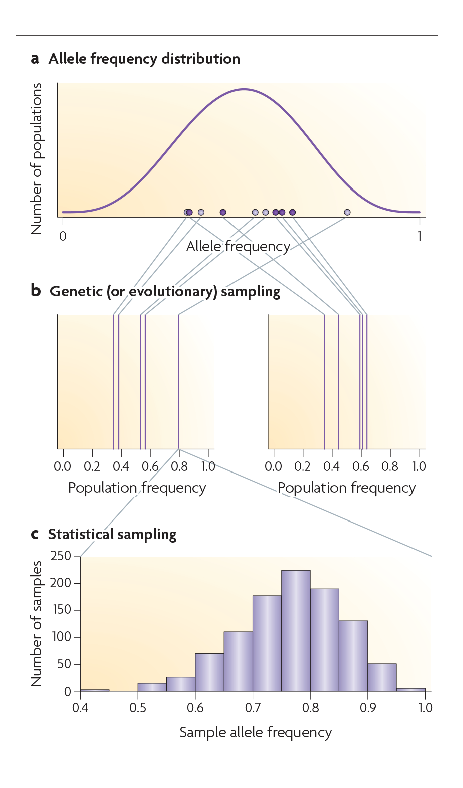
\includegraphics[height=0.9\textheight]{sampling.eps}
\end{center}
\vfill\eject
}

\myslide{
\heading{$F$-statistics: an important limitation}

$F$-statistics are great, \emphasis{but using them requires us to
  specify which individuals belong to which populations before we
  start the analysis}.

\emphasis{Question}: Is there a way to use the data we have to tell us what
populations individuals belong to?
}

\myslide{
\heading{Individual assignment using {\tt STRUCTURE}}
  
\begin{eqnarray*}
\mbox{P}(i|k) &=& \frac{\mbox{P}(x_i|\gamma_k)}{\sum_k
  \mbox{P}(x_i|\gamma_k)} \\
x_i &=& \mbox{genotype of individual $i$} \\
\gamma_k &=& \mbox{genotype frequencies in population $k$}
\end{eqnarray*}
For example, if $A_1A_1$ is labeled as $1$, $A_1A_2$ as $2$, $A_2A_2$
as 3, and we assume that genotypes are in Hardy-Weinberg, then
\begin{eqnarray*}
\mbox{P}((1,2,2,1,3)|(p_{k1}, p_{k2}, p_{k3}, p_{k4}, p_{k5})) = (p_{k1}^2)(2p_{k2}q_{k2})(2p_{k3}q_{k3})(p_{k4}^2)(q_{k5}^2)
\end{eqnarray*}
}

\myslide{
\heading{Using {\tt STRUCTURE} in barberry}
  
{\it Berberis thunbergii\/}
\begin{itemize}
\item 85 feral, 7 horticultural, 4 cultivated
\item 147 polymorphic AFLP markers
\end{itemize}
\begin{table}
\begin{center}
\begin{tabular}{cc}
\hline\hline
K & Mean L(K) \\
\hline
2 & -2553.2 \\
3 & {\bf -2331.9} \\
4 & -2402.9 \\
5 & -2476.3 \\
\hline
\end{tabular}
\end{center}
\caption{Mean log probability of the data for $K=2,3,4,5$ in the {\it
    Berberis thunbergii\/} data}
\end{table}
}

\myslide{
\heading{Using {\tt STRUCTURE} in barberry}

  \begin{figure}
\resizebox{\textwidth}{!}{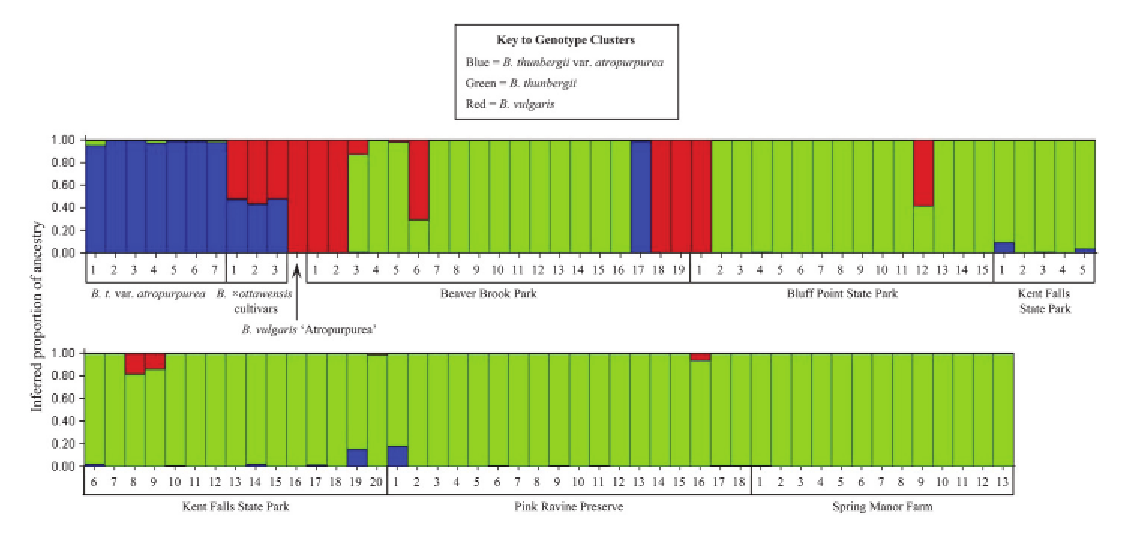
\includegraphics{lubell-structure.eps}}
\caption{Analysis of AFLP data from {\it Berberis
    thunbergii}}
\end{figure}
}

\myslide{
\heading{Using {\tt STRUCTURE} in humans}
  
\begin{itemize}

\item Human Genome Diversity Cell Line Panel (HGDP-CEPH)

\item 1056 individuals, 52 geographic populations, 377 autosomal
  microsatellite loci

\end{itemize}

\begin{figure}
\resizebox{\textwidth}{!}{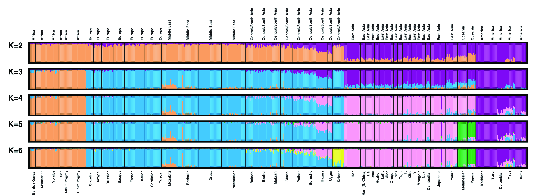
\includegraphics{HGDP-CEPH.eps}}
\end{figure}

}

\myslide{
\heading{Principal components analysis of genotypes}

Principal components analysis is a ``dimension reduction'' method, a
way of reducing a very large number of variables to a smaller, more
manageable number for interpretation and analysis.

\begin{center}
  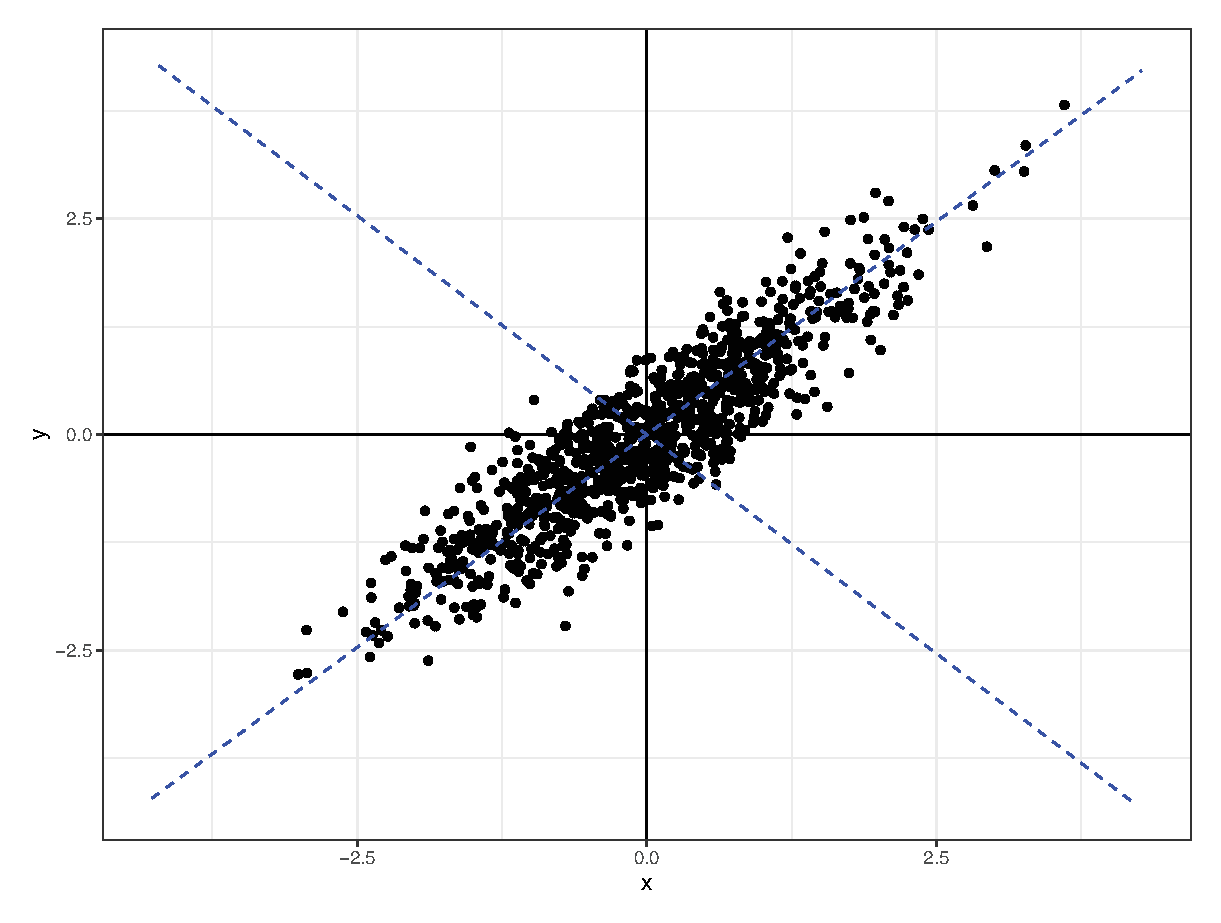
\includegraphics[height=5cm]{pca-example.eps}
\end{center}

\vfill\eject
}

\myslide{
\heading{Principal components analysis of genotypes}

3129 Europeans, 500,568 SNP loci

\begin{figure}
\begin{center}
\resizebox{0.5\textwidth}{!}{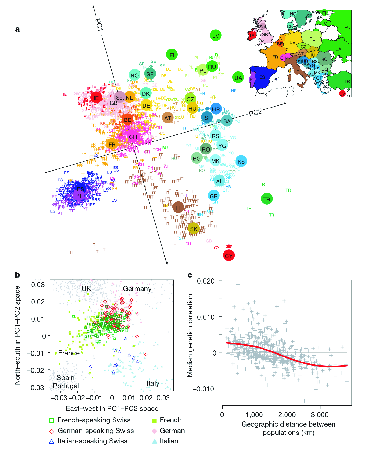
\includegraphics{human-PCA.eps}}
\end{center}
\end{figure}

}

\end{document}



